\chapter{量子化Klein-Gordon场论}
\section{K-G场的量子化}
之前我们讨论过一维弦的量子化,并且得到可以将一维弦看作无穷多独立的谐振子的叠加,出于简单我们来讨论实K-G场论。
\begin{equation}
\begin{aligned}
    \mathcal{L}_{KG}&=\frac{1}{2}(\partial_{\mu}\phi)^{2}-\frac{1}{2}m^{2}\phi^{2}\\
    \pi &=\frac{\partial \mathcal{L}}{\partial \dot{\phi}}=\dot{\phi}\\
    \mathcal{H}&=\pi\dot{\phi}-\mathcal{L}=T^{00}=\frac{1}{2}\pi^{2}+\frac{1}{2}(\nabla \phi)^{2}+\frac{1}{2}m^{2}\phi^{2}
    \end{aligned}
\end{equation}
为了使得Hamiltonian是正定的,我们需要仔细选取Lagrangian中每一项Lorentz标量前的符号。

下面我们来量子化这一理论。在非相对论量子力学中我们习惯于从Hamiltonian出发,进行正则量子化程序,
\begin{equation}
\left[\hat{q}_{\alpha},\hat{p}_{\beta}\right]=i\delta_{\alpha \beta}
\end{equation}
其他对易关系为0。

由于$\mathcal{H}$依赖于空间位置且K-G场是一个连续系统,从而有无穷多自由度,回忆在一维弦量子化时,Hamiltonian的求和在连续极限下过渡为积分,因此我们在那里对每一个独立的谐振子引入正则对易关系,相当于我们对$\mathcal{H}$引入正则对易关系。
由此我们推测,对于K-G场我们有
\begin{equation}
\label{chap3commu}
    \begin{aligned}
        \left[\phi(\vec{x}),\pi(\vec{y})\right]&=i\delta^{3}\left(\vec{x}-\vec{y}\right)\\
        \left[\phi(\vec{x}),\phi(\vec{y})\right]&=0\\
        \left[\pi(\vec{x}),\pi(\vec{y})\right]&=0\\
    \end{aligned}
\end{equation}
注意我们在这里没有引入时间变量,可以认为这些对易关系都定义在某一相同时刻\footnote{称为等时对易关系},也可以认为我们是在Schr$\ddot{\rm{o}}$dinger表象下进行讨论。

我们知道K-G场的运动方程为
\begin{equation}
   \left(\partial^{2}+m^{2}\right)\phi(\vec{x},t)=0
\end{equation}

回忆经典弦的量子化过程,我们对$\phi$进行Fourier变换,
\begin{equation}
\label{chap3fourier}
    \phi(\vec{x},t)=\int \frac{d^{3}p}{(2\pi)^{3}}e^{i\vec{p}\cdot\vec{x}}\tilde{\phi}(\vec{p},t)
\end{equation}
代入K-G方程中我们得到
\begin{equation}
\label{fourkg}
\left[ \frac{\partial^{2}}{\partial t^{2}}+\omega^{2}_{\vec{p}}\right]\tilde{\phi}(\vec{p},t)=0
\end{equation}
其中$\omega_{\vec{p}}=\sqrt{\vec{p}^{2}+m^{2}}$,这表示一个动量为$\vec{p}$,质量为$m$的粒子的能量。这与谐振子的运动方程是形式一致的。

下面我们类比一个谐振子系统\footnote{细节请看Peskin,顺便一提,我们在这一节的讨论基于等时对易关系,因此所有的计算都在某一固定的时刻进行,故不显含时间变量,或者等价地,我们的讨论都在$t=0$时刻进行。}
\begin{equation}
    H=\frac{1}{2}p^{2}+\frac{1}{2}\omega^{2}\phi^{2}
\end{equation}
我们可以将$\phi$和$\pi$用升降算符写为
\begin{equation}
\phi=\frac{1}{\sqrt{2\omega}}(a+a^{\dagger});\quad p=-i\sqrt{\frac{\omega}{2}}(a-a^{\dagger})
\end{equation}
从而正则对易关系$[\phi,p]=i$等价于
\begin{equation}
    [a,a^{\dagger}]=1
\end{equation}

对于K-G场,我们有
\begin{equation}
\begin{aligned}
H&=\int d^{3}x\left\{\frac{1}{2}\pi^{2}+\frac{1}{2}(\nabla \phi)^{2}+\frac{1}{2}m^{2}\phi^{2}\right\}\\
&=\int \frac{d^{3}p}{(2\pi)^{3}}\left[\frac{1}{2}\tilde{\pi}^{2}+\omega_{\vec{p}}^{2}\tilde{\phi}^{2}\right]
\end{aligned}
\end{equation}
其中$\tilde{\pi},\tilde{\phi}$为按照(\ref{chap3fourier})定义的通过Fourier变换得到的场变量,并且利用了$\phi$为实数场,从而满足$\tilde{\phi}^{*}(\vec{p})=\tilde{\phi}(-\vec{p})=\tilde{\phi}(\vec{p})$。

通过与谐振子形式进行对比,我们可以将场变量表示为
\begin{equation}
\label{chap3kgphi}
\begin{aligned}
    \hat{\phi}(\vec{x})&=\int \frac{d^{3}p}{(2\pi)^{3}}\frac{1}{\sqrt{2\omega_{\vec{p}}}}\left(a_{\vec{p}}(t=0)e^{i\vec{p}\cdot\vec{x}}+a^{\dagger}_{\vec{p}}(t=0)e^{-i\vec{p}\cdot\vec{x}}\right)\\
    \hat{\pi}(\vec{x})&=\int \frac{d^{3}p}{(2\pi)^{3}}(-i)\sqrt{\frac{\omega_{\vec{p}}}{2}}\left(a_{\vec{p}}(t=0)e^{i\vec{p}\cdot\vec{x}}-a^{\dagger}_{\vec{p}}(t=0)e^{-i\vec{p}\cdot\vec{x}}\right)
\end{aligned}
\end{equation}
其中$a$与$a^{\dagger}$的选择保证了$\hat{\phi},\hat{\pi}$为Hermite算符\footnote{一般的场算符不必是Hermite算符,这里是因为实K-G场满足$\phi=\phi^{*}$, 从而升级为算符后要满足$\hat{\phi}=\hat{\phi}^{\dagger}$}。

我们下面来验证,如果有
\begin{equation}
    \left[a_{\vec{p}},a^{\dagger}_{\vec{p}'}\right]=(2\pi)^{3}\delta^{3}(\vec{p}-\vec{p}')
\end{equation}
则(\ref{chap3commu})可以成立。

为方便,我们对(\ref{chap3kgphi})中第二项做变量替换$\vec{q}=-\vec{p}$,并将积分变量名从$\vec{q}$改写为$\vec{p}$可以得到
\begin{equation}
\label{chap3kgphi2}
\begin{aligned}
    \hat{\phi}(\vec{x})&=\int \frac{d^{3}p}{(2\pi)^{3}}\frac{1}{\sqrt{2\omega_{\vec{p}}}}\left(a_{\vec{p}}+a^{\dagger}_{-\vec{p}}\right)(t)e^{i\vec{p}\cdot\vec{x}}\\
    \hat{\pi}(\vec{y})&=\int \frac{d^{3}q}{(2\pi)^{3}}(-i)\sqrt{\frac{\omega_{\vec{q}}}{2}}\left(a_{\vec{q}}-a^{\dagger}_{-\vec{q}}\right)(t)e^{i\vec{q}\cdot\vec{y}}
\end{aligned}
\end{equation}
于是
\begin{equation}
\label{chap3equatime}
    \begin{aligned}
     \left[\hat{\phi}(\vec{x}),\hat{\pi}(\vec{y})\right]&=\int \frac{d^{3}p}{(2\pi)^{3}} \int \frac{d^{3}q}{(2\pi)^{3}}(-i)\frac{1}{\sqrt{2\omega_{\vec{p}}}}\sqrt{\frac{\omega_{\vec{q}}}{2}}e^{i\vec{q}\cdot\vec{y}}e^{i\vec{p}\cdot\vec{x}}\left[a_{\vec{p}}+a^{\dagger}_{-\vec{p}},a_{\vec{q}}-a^{\dagger}_{-\vec{q}}\right]\\
     &= \int \frac{d^{3}p}{(2\pi)^{3}} \int \frac{d^{3}q}{(2\pi)^{3}}(-i)\frac{1}{\sqrt{2\omega_{\vec{p}}}}\sqrt{\frac{\omega_{\vec{q}}}{2}}e^{i\vec{q}\cdot\vec{y}}e^{i\vec{p}\cdot\vec{x}}\left(-2(2\pi)^{3}\delta^{3}(\vec{p}+\vec{q})\right)\\
      &= i\int \frac{d^{3}p}{(2\pi)^{3}}\frac{\sqrt{\omega_{-\vec{p}}}}{\sqrt{\omega_{\vec{p}}}}e^{i\vec{p}\cdot(\vec{x}-\vec{y})}\delta^{3}(\vec{p}+\vec{q})\\
      &= i\int \frac{d^{3}p}{(2\pi)^{3}}e^{i\vec{p}\cdot(\vec{x}-\vec{y})}\\
      &= i\delta^{3}(\vec{x}-\vec{y})\\
 \left[\hat{\phi}(\vec{x}),\hat{\phi}(\vec{y})\right]&=\int \frac{d^{3}p}{(2\pi)^{3}} \int \frac{d^{3}q}{(2\pi)^{3}}\frac{1}{\sqrt{2\omega_{\vec{p}}}}\frac{1}{\sqrt{2\omega_{\vec{q}}}}e^{i\vec{q}\cdot\vec{y}}e^{i\vec{p}\cdot\vec{x}}\left[a_{\vec{p}}+a^{\dagger}_{-\vec{p}},a_{\vec{q}}+a^{\dagger}_{-\vec{q}}\right]\\
     &=\int \frac{d^{3}p}{(2\pi)^{3}} \int \frac{d^{3}q}{(2\pi)^{3}}\frac{1}{\sqrt{4\omega_{\vec{p}}\omega_{\vec{q}}}}e^{i\vec{q}\cdot\vec{y}}e^{i\vec{p}\cdot\vec{x}}(2\pi)^{3}\left((\delta^{3}(\vec{p}+\vec{q})-\delta^{3}(\vec{p}+\vec{q})\right)\\
     &=0\\
    \left[\hat{\pi}(\vec{x}),\hat{\pi}(\vec{y})\right]&=(-i)^{2}\int \frac{d^{3}p}{(2\pi)^{3}} \int \frac{d^{3}q}{(2\pi)^{3}}\sqrt{\frac{\omega_{\vec{p}}}{2}}\sqrt{\frac{\omega_{\vec{q}}}{2}}e^{i\vec{q}\cdot\vec{y}}e^{i\vec{p}\cdot\vec{x}}\left[a_{\vec{p}}-a^{\dagger}_{-\vec{p}},a_{\vec{q}}-a^{\dagger}_{-\vec{q}}\right]\\
     &=-\int \frac{d^{3}p}{(2\pi)^{3}} \int \frac{d^{3}q}{(2\pi)^{3}}\sqrt{\frac{\omega_{\vec{q}}\omega_{\vec{p}}}{4}}e^{i\vec{q}\cdot\vec{y}}e^{i\vec{p}\cdot\vec{x}}(2\pi)^{3}\left((\delta^{3}(\vec{p}+\vec{q})-\delta^{3}(\vec{p}+\vec{q})\right)\\
     &=0\\ 
    \end{aligned}
\end{equation}
其中利用了$\omega_{\vec{p}}=\omega_{-\vec{p}}$。

我们知道在谐振子的情况下,在使用升降算符表达场的动力学变量后,Hamiltonian有非常简单的对角表达形式$H=\omega(a^{\dagger}a+\frac{1}{2})$,在K-G场的情况下,我们下面将要看到Hamiltonian同样有非常简单的表达式。我们将$\hat{\phi}$和$\hat{\pi}$的表达式(\ref{chap3kgphi})代入
\begin{equation}
    H=\int d^{3}x\left\{\frac{1}{2}\hat{\pi}^{2}+\frac{1}{2}(\nabla \hat{\phi})^{2}+\frac{1}{2}m^{2}\hat{\phi}^{2}\right\}
\end{equation}
可以得到
\begin{equation}
\label{chap3hamilton}
    H=\int \frac{d^{3}p}{(2\pi)^{3}}\omega_{\vec{p}}\left(a^{\dagger}_{\vec{p}}a_{\vec{p}}+\frac{1}{2}\left[a_{\vec{p}},a^{\dagger}_{\vec{p}}\right]\right)
\end{equation}
其中第二项正比于$\delta^{3}(0)$,这是一个无穷大的常数,记这一项为$E_{0}$,事实上这一项来自于每一项的零点能$\frac{\omega_{\vec{p}}}{2}$的级数和。我们将这个无穷大常数的能量称为真空能,所谓真空,在场论中特指一个体系的基态。对于一维谐振子,我们有$a\ket{0}=0$,在场论中,与谐振子的情况类似,我们要求基态满足$a_{\vec{p}}\ket{0}=0$对于任意的$\vec{p}$都成立。从而我们有
\begin{equation}
    H\ket{0}=E_{0}\ket{0}
\end{equation}
因此真空$\ket{0}$具有无穷大的能量,幸运的是,由于我们能够测量的是与基态的能量差而非能量的绝对值,因此我们可以重新定义基态\footnote{类似于我们可以任意选取测量一个人身高的起算点,但是只有从头到脚的距离差才是有物理意义的}(平移一个无穷大常数)使得
\begin{equation}
    H\ket{0}=0
\end{equation}
从而我们可以忽略掉(\ref{chap3hamilton})中的无穷大常数项。省略掉这一项后,我们再次得到了对角形式的Hamiltonian。在技术上,我们上面所做的忽略掉一个无穷大常数的行为称为正则排序,即将湮灭算符强行排列到产生算符右侧,从而由于对易关系而出现在(\ref{chap3hamilton})的无穷大常数项就不再存在。真空能是0还是无穷大,对于不考虑引力效应的情况下是不会产生问题的,但是如果我们考虑广义相对论效应,根据场方程,真空能量会对空间的曲率产生影响,从而真空能的取值会产生可观测效应,这在量子引力相关的课题中是一个很深刻的问题,我们这门课只局限在平直的时空,因此今后我们可以忽略掉真空能而不影响我们此刻所关心的物理。

我们上面的讨论广泛利用了谐振子于K-G场的相似性,这再次印证了量子场论可以看作无穷多独立谐振子的联合。
\section{K-G场论的能谱}
所谓能谱,即理论的所有能量本征态。我们在上一节中定义了K-G场论的基态,并且得到了忽略掉真空能的K-G场的Hamiltonian
\begin{equation}
    H=\int \frac{d^{3}p}{(2\pi)^{3}}\omega_{\vec{p}}a^{\dagger}_{\vec{p}}a_{\vec{p}}
\end{equation}

在讨论K-G理论的激发态之前,我们仍然先回忆谐振子中Hamiltonian与升降算符的对易关系:
\begin{equation}
\begin{aligned}
    \left[H,a^{\dagger}\right]&=\omega a^{\dagger}\\
    \left[H,a\right]&=-\omega a\\
    \end{aligned}
\end{equation}
基于这一关系,我们可以证明$\ket{n}=(a^{\dagger})^{n}\ket{0}$为能量本征态。在场论中,我们也有类似的关系
\begin{equation}
\begin{aligned}
    \left[H,a^{\dagger}_{\vec{p}}\right]&=\int \frac{d^{3}q}{(2\pi)^{3}}\omega_{\vec{q}}\left[a^{\dagger}_{\vec{q}}a_{\vec{q}},a^{\dagger}_{\vec{p}}\right]\\
    &=\int d^{3}q\omega_{\vec{q}}a^{\dagger}_{\vec{q}}\delta^{3}(\vec{p}-\vec{q})\\
        &=\omega_{\vec{p}}a^{\dagger}_{\vec{p}}
    \end{aligned}
\end{equation}
同理我们有
\begin{equation}
    \left[H,a_{\vec{p}}\right]=-\omega_{\vec{p}}a_{\vec{p}}
\end{equation}

下面我们构造单粒子态$a_{\vec{p}}^{\dagger}\ket{0}$,
\begin{equation}
    Ha_{\vec{p}}^{\dagger}\ket{0}=\left[H,a_{\vec{p}}^{\dagger}\right]=\omega_{\vec{p}}a_{\vec{p}}^{\dagger}\ket{0}
\end{equation}
其中第一个等号利用了$H\ket{0}=0$。
由此可见,单粒子态是能量本征态,其本征值为$\omega_{p}=\sqrt{p^{2}+m^{2}}$。
类似地,我们也有
\begin{equation}
    H\left(a_{\vec{p}}^{\dagger}a_{\vec{q}}^{\dagger}\ket{0}\right)=\left[H,a_{\vec{p}}^{\dagger}a_{\vec{q}}^{\dagger}\right]\ket{0}=a_{\vec{p}}^{\dagger}\left[H,a_{\vec{q}}^{\dagger}\right]\ket{0}+\left[H,a_{\vec{p}}^{\dagger}\right]a_{\vec{q}}^{\dagger}\ket{0}=(\omega_{\vec{p}}+\omega_{\vec{q}})a_{\vec{p}}^{\dagger}a_{\vec{q}}^{\dagger}\ket{0}
\end{equation}
我们称这样的态为双粒子态,可以类似得到三粒子态、多粒子态等,用归纳法可以证明对于形如
\begin{equation}
    \prod\limits_{i=1}\limits^{n}a^{\dagger}_{\vec{p}_{i}}\ket{0}
\end{equation}
的态,其本征值为
\begin{equation}
\sum\limits_{i=1}\limits^{n} \omega_{\vec{p}_{i}}
\end{equation}

我们之前在(\ref{noetherEP})中得到了动量算符为
\begin{equation}
    \vec{P}=\int d^{3}x T^{0i}=-\int d^{3}x\;\pi\nabla \phi
\end{equation}
将其提升为算符,并利用(\ref{chap3kgphi2})我们可以得到
\begin{equation}
\label{chap3momenoper}
    \hat{P}=\int d^{3}x\;\vec{p}a_{\vec{p}}^{\dagger}a_{\vec{p}}
\end{equation}
由于$\vec{p}$是奇函数,因此我们在动量的情况下不会遇到零点能类似的问题。由于$\vec{p}$是一个对易的c数,因此完全平行于能量的情况,我们有
\begin{equation}
\begin{aligned}
\left[\hat{P},a_{\vec{p}}^{\dagger}\right]=\vec{p}a_{\vec{p}}\\
    \left[\hat{P},a_{\vec{p}}\right]=-\vec{p}a_{\vec{p}}\\
    \end{aligned}
\end{equation}
对于形如
\begin{equation}
    \prod\limits_{i=1}\limits^{n}a^{\dagger}_{\vec{p}_{i}}\ket{0}
\end{equation}
的态,其本征值为
\begin{equation}
\sum\limits_{i=1}\limits^{n}\vec{p}_{i}
\end{equation}
因此$n$粒子态$\prod\limits_{i=1}\limits^{n}a^{\dagger}_{\vec{p}_{i}}\ket{0}$是能量和动量的共同本征态,其能量与动量分别为各个产生算符的能量和动量之和,这也符合我们对于能量和动量是广延量的直觉。综上,我们可以认为$a^{\dagger}_{\vec{p}}\ket{0}$表示一个能量为$\omega_{\vec{p}}=\sqrt{\vec{p}^{2}+m^{2}}$,动量为$\vec{p}$的粒子,由于粒子是同一个场的激发态,因此K-G场激发产生的粒子都是全同粒子。
上面的讨论也为我们提供了理解为什么量子场论是无穷多自由度理论的一个角度:因为$a^{\dagger}_{\vec{p}}$算符的存在,我们可以构造出任意多粒子数的态。

\section{Bose-Einstein统计}
从量子场论的角度来看,导致Bose-Einstein统计的原因在于我们在量子化K-G理论时,利用了
\begin{equation}
\label{bosen1}
    \left[a^{\dagger}_{\vec{p}},a^{\dagger}_{\vec{q}}\right]=0
\end{equation}
考察一个双粒子态
\begin{equation}
    a_{\vec{p}}^{\dagger}a_{\vec{q}}^{\dagger}\ket{0}=\ket{\vec{p},\vec{q}}
\end{equation}
由于对易关系(\ref{bosen1}),我们有
\begin{equation}
    a_{\vec{p}}^{\dagger}a_{\vec{q}}^{\dagger}\ket{0}= a_{\vec{q}}^{\dagger}a_{\vec{p}}^{\dagger}\ket{0}=\ket{\vec{p},\vec{q}}=\ket{\vec{q},\vec{p}}
\end{equation}
即交换两个玻色子,物理态不变。

此外,我们也可以理解Bose-Einstein凝聚,这一现象指的是在同一个态上可以存在多个粒子,从场论角度看,这表明存在形如$(a^{\dagger}_{\vec{p}})^{n}\ket{0}$的态。

后面我们会看到,Fermi-Dirac统计则来自于反对易关系
\begin{equation}
\label{fermi1}
    \left\{a^{\dagger}_{\vec{p}},a^{\dagger}_{\vec{q}}\right\}=0
\end{equation}
这将导致
\begin{equation}
    \left(a^{\dagger}_{\vec{p}}\right)^{2}=0
\end{equation}
从而
\begin{equation}
    \left(a^{\dagger}_{\vec{p}}\right)^{2}\ket{0}=0
\end{equation}
这就是Pauli不相容原理。

下面来讨论单粒子态的归一化问题。我们根据上面的讨论,我们知道$\ket{\vec{p}}\propto a^{\dagger}_{\vec{p}}\ket{0}$,其中对于真空态我们选取
\begin{equation}
    \braket{0}{0}=1
\end{equation}

通常在非相对论量子力学中,我们会选取$\braket{\vec{p}}{\vec{q}}=(2\pi)^{3}\delta^{3}(\vec{p}-\vec{q})$,然而这一选择并不是Lorentz不变的,这是因为三维delta函数相当于具有体积的量纲,存在Lorentz收缩效应,三维体积不是Lorentz不变的。在相对论量子力学中,我们更喜欢Lorentz不变的量,因此我们需要重新选取归一化系数,使得$\braket{\vec{p}}{\vec{q}}$是Lorentz不变的。

我们考虑动量为$\vec{p}$的单粒子态,在沿着$z$轴的boost下,我们有
\begin{equation}
\begin{aligned}
p'_{3}&=\gamma(p_{3}+\beta E)\\
E'&=\gamma(E+\beta p_{3})
\end{aligned}
\end{equation}
则在新的参考系中
\begin{equation}
\begin{aligned}
    \delta^{3}(\vec{p}'-\vec{q}')&=\frac{1}{\left|dp'_{3}/dp_{3}\right|}\delta^{3}(\vec{p}-\vec{q})
    \end{aligned}
\end{equation}
其中利用了$\delta(f(x)-f(x_{0}))=\frac{1}{\left|f'(x_{0})\right|}\delta(x-x_{0})$,并将$\vec{p}'$看作$\vec{p}$的函数,在我们所考虑的沿$z$轴的boost的情况下,只有第三分量的导数$\frac{dp'_{3}}{dp_{3}}$是非平凡的。
于是我们有
\begin{equation}
\begin{aligned}
    \delta^{3}(\vec{p}-\vec{q})&=\left|\frac{dp'_{3}}{dp_{3}}\right|\delta^{3}(\vec{p}'-\vec{q}')\\
    &=\gamma\left|1+\beta \frac{dE}{dp_{3}}\right|\delta^{3}(\vec{p}'-\vec{q}')\\
     &=\gamma\left|1+\beta \frac{p_{3}}{E}\right|\delta^{3}(\vec{p}'-\vec{q}')\\
      &=\left|\frac{E'}{E}\right|\delta^{3}(\vec{p}'-\vec{q}')\\
       &=\frac{E'}{E}\delta^{3}(\vec{p}'-\vec{q}')\\
    \end{aligned}
\end{equation}
其中利用了
\begin{equation}
    \begin{aligned}
        \frac{dE}{dp_{3}}=\frac{d\sqrt{p_{1}^{2}+p_{2}^{2}+p_{3}^{2}+m^{2}}}{dp_{3}}=\frac{p_{3}}{E}
    \end{aligned}
\end{equation}
于是
\begin{equation}
    E\delta^{3}(\vec{p}-\vec{q})=E'\delta^{3}(\vec{p}'-\vec{q}')
\end{equation}
在沿$z$轴的boost下不变,对于其他两个方向的boost我们也有同样的结果,因此$ E\delta^{3}(\vec{p}-\vec{q})$是一个Lorentz不变量。

基于上面的结果,我们定义Lorentz不变的归一化条件
\begin{equation}
    \braket{\vec{p}}{\vec{q}}=2E_{\vec{p}}(2\pi)^{3}\delta^{3}(\vec{p}-\vec{q})
\end{equation}
其中因子2是一种传统。
这相当于选取\footnote{出于粒子性的考虑,我们记$\omega_{\vec{p}}$为$E_{\vec{p}}$}
\begin{equation}
    \ket{\vec{p}}=\sqrt{2E_{\vec{p}}}a^{\dagger}_{\vec{p}}\ket{0}
\end{equation}
事实上,利用真空态的归一化约定,我们有
\begin{equation}
\begin{aligned}
     \braket{\vec{p}}{\vec{q}}&=\sqrt{2E_{\vec{p}}}\sqrt{2E_{\vec{q}}}\bra{0}a_{\vec{p}}a^{\dagger}_{\vec{q}}\ket{0}\\
     &=\sqrt{2E_{\vec{p}}}\sqrt{2E_{\vec{q}}}\bra{0}a^{\dagger}_{\vec{q}}a_{\vec{p}}+(2\pi)^{3}\delta^{3}(\vec{p}-\vec{q})\ket{0}\\
     &=\sqrt{2E_{\vec{p}}}\sqrt{2E_{\vec{q}}}(2\pi)^{3}\delta^{3}(\vec{p}-\vec{q})\braket{0}{0}\\
     &=2E_{\vec{p}}(2\pi)^{3}\delta^{3}(\vec{p}-\vec{q})
     \end{aligned}
\end{equation}

最后我们来讨论一下场算符的物理意义。我们已经知道$a_{\vec{p}}$和$a^{\dagger}_{\vec{p}}$分别表示湮灭和产生一个具有确定能量和动量的单粒子态,对于场本身,我们考察
\begin{equation}
\label{chap301}
\begin{aligned}
    \phi(\vec{x})\ket{0}&=\int \frac{d^{3}p}{(2\pi)^{3}}\frac{1}{\sqrt{2E_{\vec{p}}}}\left(a_{\vec{p}}e^{i\vec{p}\cdot\vec{x}}+a^{\dagger}_{\vec{p}}e^{-i\vec{p}\cdot\vec{x}}\right)\ket{0}\\
    &=\int \frac{d^{3}p}{(2\pi)^{3}}\frac{1}{\sqrt{2E_{\vec{p}}}}e^{-i\vec{p}\cdot\vec{x}}a^{\dagger}_{\vec{p}}\ket{0}\\
    &=\int \frac{d^{3}p}{(2\pi)^{3}}\frac{1}{2E_{\vec{p}}}e^{-i\vec{p}\cdot\vec{x}}\ket{\vec{p}}\\
    \end{aligned}
\end{equation}
在非相对论量子力学中,我们有
\begin{equation}
\label{chap302}
    \ket{\vec{x}}=\int \frac{d^{3}p}{(2\pi)^{3}}e^{-i\vec{p}\cdot\vec{x}}\ket{\vec{p}}
\end{equation}
(\ref{chap301})与(\ref{chap302})的表达式非常相似,考虑到$E=\sqrt{\vec{p}^{2}+m^{2}}\xrightarrow{\vec{p}\ll m}m$,从而在非相对论极限下,两者只相差一个常数因子,从而起码在非相对论的情况下,我们可以将$\phi(\vec{x})\ket{0}$诠释成位于$\vec{x}$的一个粒子。必须要强调的是,在量子场论中,$\vec{x},\;t$永远都不是算符,原则上没有$\ket{\vec{x}}$的概念,$\vec{x}$在场论中只充当运动学变量的连续指标的作用\footnote{历史上二次量子化的混淆也部分来自于这一点,当我们考虑一个单粒子量子力学并对波函数进行二次量子化时,隐含了将坐标$\vec{x}$当作算符来处理}。

我们可以通过计算下列的矩阵元来进一步证实我们对场算符的物理诠释
\begin{equation}
\begin{aligned}
    \bra{0}\phi(\vec{x})\ket{\vec{p}}&=\bra{0}\int \frac{d^{3}q}{(2\pi)^{3}}\frac{1}{\sqrt{2E_{\vec{q}}}}\left(a_{\vec{q}}e^{i\vec{q}\cdot\vec{x}}+a^{\dagger}_{\vec{q}}e^{-i\vec{q}\cdot\vec{x}}\right)\sqrt{2E_{\vec{p}}}a^{\dagger}_{\vec{p}}\ket{0}\\
    &=e^{i\vec{p}\cdot\vec{x}}
    \end{aligned}
\end{equation}
与非相对论量子力学中$\bra{\vec{x}}\ket{\vec{p}}=e^{i\vec{p}\cdot\vec{x}}$相\textbf{类比},我们可以得到结论,算符$\phi(\vec{x})$在位置$\vec{x}$处产生一个粒子。值得注意的是,我们现在的讨论都局限在自由场论,在相互作用场论中,一个场算符可以产生多个粒子。
\section{Heisenberg表象下的Klein-Gordon场}
我们之前讨论的量子化是在$t=0$时刻进行的等时量子化,即我们是在Schr$\ddot{o}$dinger表象下进行讨论,在这一绘景下,算符是不含时间依赖的,而态是时间依赖的。由于算符和态本身都不是物理可观测的,它们形成的矩阵元才是物理可观测量,因此我们有一定的自由度将时间依赖关系从态转移到算符,这样的表象称之为Heisenberg表象。不同的表象下我们最终得到的物理是完全一样的。

我们现在需要从$\phi(\vec{x},t=0)$过渡到$\phi(\vec{x},t)$,这需要借助于时间演化算符。对于两个表象下的算符,我们有关系
\begin{equation}
    O_{H}(x)=O_{H}(\vec{x},t)=e^{iHt}O_{S}(\vec{x},t=0)e^{-iHt}
\end{equation}
于是我们有\footnote{由于我们这门课主要在Heisenberg表象下进行讨论,因此常常省略掉下标$H$}
\begin{equation}
\label{chap3fieldtime}
    \phi_{H}(x)=\phi_{H}(\vec{x},t)=e^{iHt}\phi(\vec{x},t=0)e^{-iHt}
\end{equation}
我们知道Heisenberg运动方程为
\begin{equation}
    i\partial_{t}O_{H}=[O_{H},H]
\end{equation}
于是我们可以得到Heisenberg表象下场算符的时间依赖关系
\begin{equation}
\label{chap3Heise}
    \begin{aligned}
        i\frac{\partial}{\partial t}\phi(\vec{x},t)&=\left[\phi(\vec{x},t), \int d^{3}y\left\{\frac{1}{2}\pi^{2}(\vec{y},t)+\frac{1}{2}(\nabla \phi(\vec{y},t))^{2}+\frac{1}{2}m^{2}\phi^{2}(\vec{y},t)\right\}\right]\\
        &=\int d^{3}y\left(i\delta^{3}(\vec{x}-\vec{y})\pi(\vec{y},t)\right)\\
        &=i\pi(\vec{x},t)\\
        i\frac{\partial}{\partial t}\pi(\vec{x},t)&=\left[\pi(\vec{x},t), \int d^{3}y\left\{\frac{1}{2}\pi^{2}(\vec{y},t)+\frac{1}{2}(\nabla \phi(\vec{y},t))^{2}+\frac{1}{2}m^{2}\phi^{2}(\vec{y},t)\right\}\right]\\
         &=\frac{1}{2}\int d^{3}y\left[\pi(\vec{x},t),(\nabla \phi(\vec{y},t))^{2}+m^{2}\phi^{2}(\vec{y},t)\right]\\
          &=\int d^{3}y\left\{\nabla\phi(\vec{y},t)\cdot\left[\pi(\vec{x},t),\nabla \phi(\vec{y},t)\right]-im^{2}\delta^{3}(\vec{x}-\vec{y})\phi(\vec{y},t)\right\}\\
            &=-i\int d^{3}y\left\{\nabla\phi(\vec{y},t)\cdot\nabla\delta^{3}(\vec{x}-\vec{y})+m^{2}\delta^{3}(\vec{x}-\vec{y})\phi(\vec{y},t)\right\}\\
        &=-i\int d^{3}y\left(\delta^{3}(\vec{x}-\vec{y})(-\nabla^{2}+m^{2})\phi(\vec{y},t)\right)\\
        &=i(\nabla^{2}-m^{2})\phi(\vec{x},t)\\
    \end{aligned}
\end{equation}
由于我们目前只有等时对易关系,因此在上面的计算中,我们需要选取与场变量定义在同一时刻的Hamiltonian,由于Hamiltonian是一个守恒荷,因此它不随着时间演化,所以我们的选取是合法的。

利用上面两个算符等式我们可以得到
\begin{equation}
\label{chap3operkg}
    \frac{\partial^{2}}{\partial^{2}t}\hat{\phi}=(\nabla^{2}-m^{2})\hat{\phi}
\end{equation}
为了强调这是一个算符等式,我们暂时恢复了算符记号。我们可以看到(\ref{chap3operkg})与K-G方程形式相同,因此我们得到结论,在量子水平,场算符仍然满足K-G方程,这是一个非常普适的结论,在其他自由场论中,这一结论一般也是成立的。

在$t=0$时刻,我们有场算符的Fourier展开
\begin{equation}
     \phi(\vec{x})=\int \frac{d^{3}p}{(2\pi)^{3}}\frac{1}{\sqrt{2E_{\vec{p}}}}\left(a_{\vec{p}}(t=0)e^{i\vec{p}\cdot\vec{x}}+a^{\dagger}_{\vec{p}}(t=0)e^{-i\vec{p}\cdot\vec{x}}\right)
\end{equation}
对于任意$t$时刻,我们想要知道场算符是否仍有类似的展开,这要求我们计算$e^{iHt}\phi(\vec{x},t=0)e^{-iHt}$,即我们需要计算$a_{\vec{p}}(t)\doteq e^{iHt}a_{\vec{p}}(t=0)e^{-iHt}$和$a_{\vec{p}}^{\dagger}(t)\doteq e^{iHt}a_{\vec{p}}^{\dagger}(t=0)e^{-iHt}$
利用Hamiltonian的表达式
\begin{equation}
    H=\int \frac{d^{3}p}{(2\pi)^{3}}\omega_{\vec{p}}a^{\dagger}_{\vec{p}}a_{\vec{p}}
\end{equation}
我们有
\begin{equation}
    \begin{aligned}
    \left[H,a_{\vec{p}}\right]&=-E_{\vec{p}}a_{\vec{p}}\\
    \left[H,a_{\vec{p}}^{\dagger}\right]&=E_{\vec{p}}a_{\vec{p}}^{\dagger}\\
    \end{aligned}
\end{equation}
从而
\begin{equation}
    \begin{aligned}
    H^{n}a_{\vec{p}}&=H^{n-1}Ha_{\vec{p}}=H^{n-1}a_{\vec{p}}(H-E_{\vec{p}})=a_{\vec{p}}(H-E_{\vec{p}})^{n}\\
     H^{n}a_{\vec{p}}^{\dagger}&=H^{n-1}Ha_{\vec{p}}^{\dagger}=H^{n-1}a^{\dagger}_{\vec{p}}(H+E_{\vec{p}})=a^{\dagger}_{\vec{p}}(H+E_{\vec{p}})^{n}\\
    \end{aligned}
\end{equation}
于是
\begin{equation}
\label{time1}
    \begin{aligned}
   a_{\vec{p}}(t)&\doteq e^{iHt}a_{\vec{p}}(t=0)e^{-iHt}\\
   &=\sum\limits_{k=1}\limits^{\infty}\frac{1}{n!}(iHt)^{k}a_{\vec{p}}(t=0)e^{-iHt}\\
   &=\sum\limits_{k=1}\limits^{\infty}\frac{1}{n!}(it)^{k}a_{\vec{p}}(t=0)(H-E_{\vec{p}})^{k}e^{-iHt}\\
   &=a_{\vec{p}}(t=0)e^{i(H-E_{\vec{p}})t}e^{-iHt}\\
   &=a_{\vec{p}}(t=0)e^{-iE_{\vec{p}}t}\\
    \end{aligned}
\end{equation}
其中最后一个等号利用了Baker-Campbell-Hausdorff-公式及$H$与$H-E_{\vec{p}}$对易。

完全类似地,我们有
\begin{equation}
\label{time2}
    \begin{aligned}
        a_{\vec{p}}^{\dagger}(t)&\doteq e^{iHt}a_{\vec{p}}^{\dagger}(t=0)e^{-iHt}\\
   &=a_{\vec{p}}^{\dagger}(t=0)e^{iE_{\vec{p}}t}
    \end{aligned}
\end{equation}
利用(\ref{time1})和(\ref{time2})我们有
\begin{equation}
\label{chap3phi4D}
\begin{aligned}
    \phi(x)&=e^{iHt}\phi(\vec{x},t=0)e^{-iHt}\\
    &=\int \frac{d^{3}p}{(2\pi)^{3}}\frac{1}{\sqrt{2E_{\vec{p}}}}\left(a_{\vec{p}}(t)e^{i\vec{p}\cdot\vec{x}}+a^{\dagger}_{\vec{p}}(t)e^{-i\vec{p}\cdot\vec{x}}\right)\\
    &=\int \frac{d^{3}p}{(2\pi)^{3}}\frac{1}{\sqrt{2E_{\vec{p}}}}\left(a_{\vec{p}}e^{i\vec{p}\cdot\vec{x}-iE_{\vec{p}}t}+a^{\dagger}_{\vec{p}}e^{-i\vec{p}\cdot\vec{x}+iE_{\vec{p}}t}\right)\\
      &=\int \frac{d^{3}p}{(2\pi)^{3}}\frac{1}{\sqrt{2E_{\vec{p}}}}\left.\left(a_{\vec{p}}e^{-ipx}+a^{\dagger}_{\vec{p}}e^{ipx}\right)\right|_{p^{0}=E_{\vec{p}}=\sqrt{\vec{p}^{2}+m^{2}}}\\
    \end{aligned}
\end{equation}
根据(\ref{chap3Heise})我们可以得到正则动量
\begin{equation}
\pi(x)=\frac{\partial}{\partial t}\phi(x)=-i\int \frac{d^{3}p}{(2\pi)^{3}}\sqrt{\frac{E_{\vec{p}}}{2}}\left.\left(a_{\vec{p}}e^{-ipx}-a^{\dagger}_{\vec{p}}e^{ipx}\right)\right|_{p^{0}=E_{\vec{p}}=\sqrt{\vec{p}^{2}+m^{2}}}
\end{equation}
这样就得到了在Heisenberg表象下任意时刻场算符的平面波分解。我们称含有$e^{-iE_{\vec{p}}t}$的项为正频部分,含有$e^{iE_{\vec{p}}t}$的项为负频部分,其中正负的规定来自Schr$\ddot{o}$dinger的能量本征态的形式解:对于方程$i\frac{\partial}{\partial t}\psi=H\psi=E\psi$,其解满足$\psi \propto e^{-iEt}$,由于$E_{\vec{p}}$总是正的,因此$e^{-iE_{\vec{p}}}$的项即对应正频部分,$e^{iE_{\vec{p}}}=e^{-i(-E_{\vec{p}})}$对应负频部分。在场论中,湮灭算符属于正频部分、产生部分属于负频部分是非常普遍的一种搭配方式。由于$\hat{\phi}$满足K-G方程,因此其具有负频率解,但是我们前面的构造已经给出$a_{\vec{p}}^{\dagger}\ket{0}$是具有正能量$E_{\vec{p}}$的态,因此尽管其具有负的频率,但是此时不存在负能解问题。作为一个实标量场论,K-G场满足$\phi=\phi^{\dagger}$,而对于一个非实的场论,如复K-G场论,其一般的满足运动方程的平面波分解具有形式
\begin{equation}
\label{chap3CKGfenjie}
    \phi(x)=\int \frac{d^{3}p}{(2\pi)^{3}}\frac{1}{\sqrt{2E_{\vec{p}}}}\left(a_{\vec{p}}e^{-ipx}+b^{\dagger}_{\vec{p}}e^{ipx}\right)
\end{equation}
在Dirac场论中我们将详细讨论这类平面波分解的物理意义,事实上,如果我们将$a^{\dagger}_{\vec{p}}$的效果诠释成产生一个动量为$\vec{p}$的粒子,则$b^{\dagger}_{\vec{p}}$表示产生一个动量为$\vec{p}$的反粒子,尽管反粒子有相反的频率,其能量仍然是正的,因此在量子场论中,只存在正能态的产生和湮灭,湮灭一个正能量粒子在效果上类似于产生一个负能粒子,但是由于真空态的存在,这一过程不能无限进行下去,因此系统的能级有下限,不会变成负值。

与(\ref{time1})和(\ref{time2})类似,我们对于场的空间变量部分有
\begin{equation}
\begin{aligned}
    e^{-i\vec{P}\cdot\vec{x}}a_{\vec{p}} e^{i\vec{P}\cdot\vec{x}}&=a_{\vec{p}} e^{i\vec{p}\cdot\vec{x}}\\
     e^{-i\vec{P}\cdot\vec{x}}a^{\dagger}_{\vec{p}} e^{i\vec{P}\cdot\vec{x}}&=a^{\dagger}_{\vec{p}} e^{-i\vec{p}\cdot\vec{x}}\\
    \end{aligned}
\end{equation}
其中$\vec{P}$按(\ref{chap3momenoper})定义。从而类似于(\ref{chap3fieldtime}),我们有
\begin{equation}
\label{chap3trans}
    \phi(x)=e^{iHt-i\vec{P}\cdot\vec{x}}\phi(0)e^{-iHt+i\vec{P}\cdot\vec{x}}=e^{iPx}\phi(0)e^{-iPx}
\end{equation}
其中$P^{\mu}=(H,\vec{P})$是一个算符。在场论中,时空坐标只是一个标签,只要我们知道原点处的值,就可以通过平移得到任意时空处的值。注意到真空是具有平移不变性的,即
\begin{equation}
    e^{i\hat{P}x}\ket{0}=\left(1+\sum\limits_{k=1}\limits^{\infty}(ix)^{k}(\hat{P})^{k}\right)\ket{0}=\ket{0}
\end{equation}

由以上讨论可见,场$\phi(x)$一方面能产生或湮灭一个粒子态($a_{\vec{p}},a^{\dagger}_{\vec{p}}$),另一方面又是K-G波动方程的解($e^{\pm ipx}$),因此量子场论完美地统一描述了波粒二象性。
\section{关联函数和因果性}
我们在这一节中将讨论在场论中因果性是如何被保证的。为了这一目的,我们需要定义两点关联函数\footnote{此后如不特殊说明,我们均在Heisenberg表象下讨论问题}\footnote{我们也可以定义一点关联函数$\bra{0}\phi(x)\ket{0}=0$,即场的真空期待值是0,但这只是一个多次测量之后得到的平均值,并不意味着真空中场的测量值总是0。在对称性自发破缺相关的理论中,由于真空具有的对称性小于Lagrangian具有的对称性,场的真空期望值可以不为0,这一部分知识可以在规范场论中学习到。}
\begin{equation}
    D(x-y)=\bra{0}\phi(x)\phi(y)\ket{0}
\end{equation}
其物理意义表示一个粒子从时空点$y$传播到时空点$x$的传播振幅,我们将(\ref{chap3phi4D})代入可以得到
\begin{equation}
    \begin{aligned}
        D(x-y)&=\bra{0}\phi(x)\phi(y)\ket{0}\\
        &=\bra{0}\int \frac{d^{3}pd^{3}q}{(2\pi)^{6}}\frac{1}{\sqrt{4E_{\vec{p}}E_{\vec{q}}}}\left(a_{\vec{p}}e^{-ipx}+a^{\dagger}_{\vec{p}}e^{ipx}\right)\left(a_{\vec{q}}e^{-iqy}+a^{\dagger}_{\vec{q}}e^{iqy}\right)\ket{0}\\
        &=\int \frac{d^{3}pd^{3}q}{(2\pi)^{6}}\frac{1}{\sqrt{4E_{\vec{p}}E_{\vec{q}}}}e^{iqy-ipx}\bra{0}a_{\vec{p}}a^{\dagger}_{\vec{q}}\ket{0}\\
         &=\int \frac{d^{3}pd^{3}q}{(2\pi)^{6}}\frac{1}{\sqrt{4E_{\vec{p}}E_{\vec{q}}}}e^{iqy-ipx}(2\pi)^{3}\delta^{3}(\vec{p}-\vec{q})\\
         &=\int \frac{d^{3}p}{(2\pi)^{3}}\frac{1}{2E_{\vec{p}}}e^{-ip(x-y)}\\
    \end{aligned}
\end{equation}
显然相位因子$e^{-ip(x-y)}$是Lorentz不变的,对于积分测度,我们有如下等式
\begin{equation}
    \begin{aligned}
       &\int \frac{d^{4}p}{(2\pi)^{4}}(2\pi)\delta(p^{2}-m^{2})\theta(p^{0})\\
       =&\int \frac{d^{3}p}{(2\pi)^{3}}\int dp^{0}\delta(p^{2}-m^{2})\theta(p^{0})\\
       =&\int \frac{d^{3}p}{(2\pi)^{3}}\int\limits_{0}\limits^{\infty} dp^{0}\delta\left((p^{0})^{2}-\vec{p}^{2}-m^{2}\right)\\
       =&\int \frac{d^{3}p}{(2\pi)^{3}}\sum_{\substack{p^{0}>0;\\(p^{0})^{2}-\vec{p}^{2}-m^{2}=0}}\frac{1}{|2p^{0}|}\\
       =&\int \frac{d^{3}p}{(2\pi)^{3}}\frac{1}{2E_{\vec{p}}}
    \end{aligned}
\end{equation}
其中$\theta(t)$是Heaviside函数
\begin{equation}
    \theta(t)=\left\{
    \begin{array}{cc}
          1,\quad t> 0\\
          \frac{1}{2},\quad t=0 \\
          0,\quad t < 0
    \end{array}
    \right.
\end{equation}
由于在连续Lorentz变换下不改变$p^{0}$的符号,因此这一项是Lorentz不变的,显然$d^{4}p$与$\delta(p^{2}-m^{2})$也是Lorentz不变的,因此积分测度$\int \frac{d^{3}p}{(2\pi)^{3}}\frac{1}{2E_{\vec{p}}}$Lorentz不变,从而我们得到$D(x-y)$是一个Lorentz不变量,这一点很容易理解,因为真空和标量场算符是Lorentz不变的。

此外我们注意到,关联函数只是$x-y$的函数,即只依赖于两时空点之间的差,这一点可以由真空的平移不变性及(\ref{chap3trans})得到
\begin{equation}
    \bra{0}\phi(x)\phi(y)\ket{0}=\bra{0}e^{i\hat{P}y}\phi(x-y)e^{-i\hat{P}y}e^{i\hat{P}y}\phi(0)e^{-i\hat{P}y}\ket{0}=\bra{0}\phi(x-y)\phi(0)\ket{0}
\end{equation}

当$x-y$是类时间隔时,我们总可以找到一个特殊的参考系使得$x^{0}-y^{0}=t$而$\vec{x}=\vec{y}=0$,从而
\begin{equation}
\label{chap3222}
    \begin{aligned}
        D(x-y)&=\int \frac{d^{3}p}{(2\pi)^{3}}\frac{1}{2E_{\vec{p}}}e^{-iE_{\vec{p}}t}\\
        &=\frac{4\pi}{(2\pi)^{3}}\int_{0}^{\infty}dq\frac{q^{2}}{2\sqrt{q^{2}+m^{2}}}e^{-i\sqrt{q^{2}+m^{2}}t}\\
        &=\frac{1}{4\pi^{2}}\int_{m}^{\infty}dE\sqrt{E^{2}-m^{2}}e^{-iEt}\\
        &\sim e^{-imt} (t\rightarrow\infty)
    \end{aligned}
\end{equation}
其中第一个等号到第二个等号我们采用了球坐标,$q=|\vec{p}|$。因为类时间隔的两个事件可以存在因果联系,因此这一非零结果是可以预期的。

当$x-y$是类空间隔时,我们总可以找到一个特殊的参考系使得$x^{0}-y^{0}=0$而$\vec{x}=\vec{y}=\vec{r}$,从而
\begin{equation}
\label{chap333}
    \begin{aligned}
        D(x-y)&=\int \frac{d^{3}p}{(2\pi)^{3}}\frac{1}{2E_{\vec{p}}}e^{i\vec{p}\cdot\vec{r}}\\
        &=\frac{2\pi}{(2\pi)^{3}}\int_{0}^{\infty}dp\frac{p^{2}}{2E_{\vec{p}}}\frac{e^{ipr}-e^{-ipr}}{ipr}\\
        &=\frac{-i}{8\pi^{2}r}\int_{-\infty}^{\infty}dp\frac{pe^{ipr}}{\sqrt{p^{2}+m^{2}}}\\
    \end{aligned}
\end{equation}
与我们在(\ref{chap1calcu})中所做的计算类似,应用留数定理我们可以得到
\begin{equation}
\begin{aligned}
    D(x-y)&=\frac{-i}{8\pi^{2}r}\int_{-\infty}^{\infty}dp\frac{pe^{ipr}}{\sqrt{p^{2}+m^{2}}}\\
    &=\frac{1}{4\pi^{2}r}\int_{m}^{\infty}d\rho \frac{\rho e^{-\rho r}}{\sqrt{\rho^{2}-m^{2}}} \xrightarrow{r\rightarrow \infty}e^{-mr}
    \end{aligned}
\end{equation}
因为类空间隔的两个事件是不存在因果联系的,我们期待其关联函数是严格的0,但是事实并非如此,这是因为因果关系指的是$y$点的事件是否会对$x$点的事件产生影响,而不是粒子能否以类空的形式传播。如果两点之间可以同时测量,则它们的测量值互相独立,从而没有因果关系,否则则具有因果关系,而两个量能否同时测量是由其对易关系给出的,
\begin{equation}
\label{chap3commuta}
    \left[O_{1}(x),O_{2}(y)\right]=0
\end{equation}
其中$O_{i}$为玻色型算符,对于费米型算符,我们需要将对易关系替换成反对易关系。
因此判断因果性在场论中是否被保护我们需要考察$\left[\phi(x),\phi(y)\right]$的取值。

由于
\begin{equation}
\label{chap3realKG}
\begin{aligned}
    &\left[\phi(x),\phi(y)\right]\\
    =&\int\frac{d^{3}p}{(2\pi)^{3}\sqrt{2E_{\vec{p}}}}\int\frac{d^{3}q}{(2\pi)^{3}\sqrt{2E_{\vec{q}}}}\left[a_{\vec{p}}e^{-ipx}+a^{\dagger}_{\vec{p}}e^{ipx},a_{\vec{q}}e^{-iqy}+a^{\dagger}_{\vec{q}}e^{iqy}\right]\\
    =&\int\frac{d^{3}p}{(2\pi)^{3}}\frac{1}{2E_{\vec{p}}}\left[e^{-ip(x-y)}-e^{ip(x-y)}\right]
    \end{aligned}
\end{equation}
这是一个c数,从而我们有
\begin{equation}
     \left[\phi(x),\phi(y)\right]= \bra{0}\left[\phi(x),\phi(y)\right]\ket{0}=D(x-y)-D(y-x)
\end{equation}
这是一个Lorentz不变量。

对于类空间隔,由于$\left[\phi(x),\phi(y)\right]$是Lorentz不变量,因此我们可以选取特殊的参考系,使得$x^{0}-y^{0}=0$而$\vec{x}=\vec{y}=\vec{r}$,此时我们可以利用之前得到的场算符的等时对易关系(\ref{chap3equatime}),我们可以得到\footnote{另一种推导方式,即老师在课上所采用的方案,见Peskin。也可以在$D(x-y)$的显式表达式(\ref{chap333})中令$\vec{q}=-\vec{p}$直接验证类空间隔满足$D(x-y)=D(y-x)$。}
\begin{equation}
\left[\phi(x),\phi(y)\right]=0,\quad {\rm if}\;\; (x-y)^{2}<0
\end{equation}
这说明类空间隔的两个事件的测量是相互独立的。事实上,这一计算可以推广到任意算符,例如对于正则动量,我们有
\begin{equation}
\left[\phi(x),\pi(y)\right]=i\delta^{3}(\vec{x}-\vec{y})=0,\quad {\rm if}\;\; (x-y)^{2}<0
\end{equation}

对于类时间隔,我们选取参考系使得$x^{0}-y^{0}=t$而$\vec{x}=\vec{y}=0$
根据(\ref{chap3222})中的推导我们可以得到$D(y-x)\sim e^{imt}(t\rightarrow \infty)$,从而对类时间隔我们有
\begin{equation}
    \begin{aligned}
        \left[\phi(x),\phi(y)\right]\sim e^{-imt}-e^{imt}(t\rightarrow \infty)\neq0
    \end{aligned}
\end{equation}
这说明类时间隔的两个事件的测量不是相互独立的。

综上,我们看到场论保持了因果性。

由于K-G场是一个中性的标量场,从而$\phi(x)$是一个厄米算符,从它的平面波展开中我们可以看出,K-G场对应的标量粒子的反粒子是其自身,因此因果性带来的物理后果不是特别明显,因此我们临时考虑复K-G场论。我们在(\ref{CKG})中已经给出了这一理论的Lagrangian,并在(\ref{CKGQ})中给出了这一理论的守恒荷,由于$\phi$是复数场,它有两个自由度,我们将其写成$\phi=\phi_{1}+i\phi_{2}$,其中$\phi_{i}$都为实数场,将这一分解代入$\mathcal{L}_{CKG}$可以得到
\begin{equation}
    \mathcal{L}'_{CKG}=\partial_{\mu}\phi_{1}\partial^{\mu}\phi_{1}-m^{2}\phi_{1}\phi_{1}+\partial_{\mu}\phi_{2}\partial^{\mu}\phi_{2}-m^{2}\phi_{2}\phi_{2}
\end{equation}
这是两个彼此独立的实K-G场之和。
由于此时$\phi$不再是厄米的,
\begin{equation}
    \phi(x)=\int \frac{d^{3}p}{(2\pi)^{3}}\frac{1}{\sqrt{2E_{\vec{p}}}}\left(a_{\vec{p}}e^{-ipx}+b^{\dagger}_{\vec{p}}e^{ipx}\right)
\end{equation}
这一表达式及其物理解释已在(\ref{chap3CKGfenjie})及其前后的段落中给出,需要强调的是$a$($a^{\dagger}$)与$b$($b^{\dagger}$)算符满足相同的关系,如都会湮灭真空、产生粒子等。

将其量子化后非零的对易子只有
\begin{equation}
    \begin{aligned}
        \left[a_{\vec{p}},a^{\dagger}_{\vec{q}}\right]&=(2\pi)^{3}\delta^{3}(\vec{p}-\vec{q})\\
            \left[b_{\vec{p}},b^{\dagger}_{\vec{q}}\right]&=(2\pi)^{3}\delta^{3}(\vec{p}-\vec{q})\\
    \end{aligned}
\end{equation}
我们将$a^{\dagger}_{\vec{p}}$($a_{\vec{p}}$)与$b^{\dagger}_{\vec{p}}$($b_{\vec{p}}$)分别解释为一对互为反粒子的产生(湮灭)算符。

对于复K-G场论,
\begin{equation}
    \begin{aligned}
         &\bra{0}\left[\phi(x),\phi(y)\right]\ket{0}\\
    =&\bra{0}\phi(x)\phi(y)\ket{0}-\bra{0}\phi(y)\phi(x)\ket{0}\\
    \propto&\bra{0}ab^{\dagger}\ket{0}\\
    =&0
    \end{aligned}
\end{equation}
因此这一对易子是平庸的,我们通常更感兴趣的是
\begin{equation}
\label{chap3CKGcommu}
    \begin{aligned}
         &\bra{0}\left[\phi(x),\phi^{\dagger}(y)\right]\ket{0}\\
    =&\bra{0}\phi(x)\phi^{\dagger}(y)\ket{0}-\bra{0}\phi^{\dagger}(y)\phi(x)\ket{0}\\
    \sim &\bra{0}(a+b^{\dagger})(a^{\dagger}+b)\ket{0}+\bra{0}(a^{\dagger}+b)(a+b^{\dagger})\ket{0}\\
    \sim &\bra{0}aa^{\dagger}\ket{0}-\bra{0}bb^{\dagger}\ket{0}
    \end{aligned}
\end{equation}
上面最后两行为方便我们省略了指数因子。
根据我们在实K-G场论的情况可以知道,单纯的$\bra{0}aa^{\dagger}\ket{0}$项并不能保证对易子严格为0,因此,我们得出结论,若想在复K-G场的情况下保持因果性,必须有反粒子的存在。事实上,因果性要求对易子严格为0会给我们带来极其非平庸的结论。由于积分测度含有$\frac{1}{\sqrt{2E_{\vec{p}}}}$项,因此要想(\ref{chap3CKGcommu})中粒子$a$与反粒子$b$的振幅完全抵消,我们必须有$E_{\vec{p},a}=E_{\vec{p},b}$这要求$m_{a}=m_{b}$,即粒子与其反粒子有完全相同的质量。

综上,因果性要求:(1)每一种粒子\textbf{必须}存在反粒子,且(2)反粒子与正粒子的质量严格相等。

历史上第一个预言反粒子的存在性的人是Dirac,他从相对论量子力学的角度出发论证了正电子的存在性并很快得到了实验证实。
\section{Klein-Gordon场的传播子}
在这一节中我们将讨论两类传播子\footnote{我们将传播子、Green函数、两点关联函数视作同义词,并将交替地使用它们。},一种是推迟(retarded)传播子,一种是Feynman传播子。
在因果性中我们经常考虑的是场算符的对易子,下面我们进一步假设$x^{0}>y^{0}$,
\begin{equation}
\label{chap386}
\begin{aligned}
 \bra{0}\left[\phi(x),\phi(y)\right]\ket{0}
    &=\left.\int\frac{d^{3}p}{(2\pi)^{3}}\frac{1}{2E_{\vec{p}}}\left[e^{-ip(x-y)}-e^{ip(x-y)}\right]\right|_{p^{0}=E_{\vec{p}}=\sqrt{\vec{p}^{2}+m^{2}}}\\
    &=\int\frac{d^{3}p}{(2\pi)^{3}}\left\{\left.\frac{1}{2E_{\vec{p}}}e^{-ip(x-y)}\right|_{p^{0}=E_{\vec{p}}}+\left.\frac{1}{-2E_{\vec{p}}}e^{-ip(x-y)}\right|_{p^{0}=-E_{\vec{p}}}\right\}\\
    &=\int\frac{d^{3}p}{(2\pi)^{3}}\int \frac{dp^{0}}{2\pi i}\frac{-1}{p^{2}-m^{2}}e^{-ip(x-y)}
    \end{aligned}
    \end{equation}
    其中选择的围道如图\ref{fig2}所示
    \begin{figure}[htbp]
        \centering
        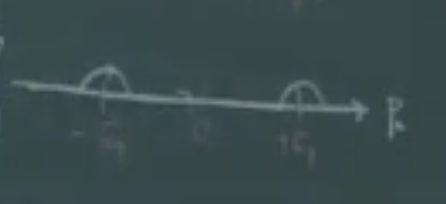
\includegraphics{img/chap3_1.png}
        \caption{(\ref{chap386})中最后一行选用的围道,当$x^{0}>y^{0}$时,为了使得大圆弧上积分为0,我们要选去圆弧经过下半平面,此时围道内有两个极点,积分结果非零,其中的负号来自于围道顺时针绕过了极点。当$x^{0}<y^{0}$时,为了大圆弧上积分结果为0,我们选取大圆弧经过上半平面,此时积分结果为0。}
        \label{fig2}
    \end{figure}
    
我们定义推迟传播子
\begin{equation}
\label{chap3retarded}
\begin{aligned}
        D_{R}(x-y)&=\theta(x^{0}-y^{0})\bra{0}\left[\phi(x),\phi(y)\right]\ket{0}\\
        &=\int_{C_{1}} \frac{d^{4}p}{(2\pi)^{4}}\frac{i}{p^{2}-m^{2}}e^{-ip(x-y)}
\end{aligned}
\end{equation}
其中$\theta(t)$为Heaviside函数,围道$C_{1}$按图(\ref{fig2})定义\footnote{这一点是值得强调的,由于我们引入的$p^{0}$的积分本身是ill-define的,事实上不同的围道选择定义了关于$p^{0}$的积分}。

下面我们简单回忆一下Green函数的基本内容。与在经典电动力学中的情况类似,我们考虑标量场,并且考虑一个有限时间区间内存在的外源$j(x)$,Lagrangian可写为
\begin{equation}
    \mathcal{L}=\frac{1}{2}(\partial_{\mu}\phi)^{2}-\frac{1}{2}m^{2}\phi^{2}+j(x)\phi(x)
\end{equation}
从而利用E-L方程我们得到含源K-G方程为
\begin{equation}
    (\partial^{2}+m^{2})\phi=j(x)
\end{equation}
在给定满足不含源K-G方程的初条件$\phi_{0}$后\footnote{因为外源只存在有限时间,我们取足够远的过去,就可以恢复之前得到的真空解(\ref{chap3phi4D}),因此不妨设$\phi_{0}$满足不含源的K-G方程},我们可以得到通解为
\begin{equation}
\label{chap3tongjie}
    \phi(x)=\phi_{0}(x)+i\int d^{4}yD_{R}(x-y)j(y)
\end{equation}
其中$D_{R}(x-y)$为经典场论中的Green函数,满足
\begin{equation}
\label{chap3st}
    (\partial^{2}+m^{2})D_{R}(x-y)=-i\delta^{4}(x-y)
\end{equation}
利用这一定义,我们可以验证通解(\ref{chap3tongjie})满足含源K-G方程:
\begin{equation}
    \begin{aligned}
    (\partial^{2}_{x}+m^{2})\phi(x)&=(\partial^{2}_{x}+m^{2})\phi_{0}(x)+i\int d^{4}y(\partial^{2}_{x}+m^{2})D_{R}(x-y)j(y)\\
    &=0+\int d^{4}y\delta^{4}(x-y)j(y)\\
    &=j(x)
    \end{aligned}
\end{equation}
其中$\partial^{2}_{x}$表示微分算符只作用于$x$变量。
直接验算可以知道,K-G场的推迟传播子(\ref{chap3retarded})也满足(\ref{chap3st})。这也可以从动量空间中看出。
从Fourier变换的定义$D_{R}(x-y)=\int \frac{d^{4}p}{(2\pi)^{4}}e^{-ip(x-y)}\tilde{D_{R}}(p)$我们可以直接从(\ref{chap3retarded})中看出,在动量空间推迟传播子的形式为
\begin{equation}
    \widetilde{D}_{R}(p)=\frac{i}{p^{2}-m^{2}}
\end{equation}
而微分算符的形式变为$-ip$,从而在动量空间,我们有
\begin{equation}
    \mathcal{F}\left[(\partial^{2}+m^{2})D_{R}(x-y)\right]=(-p^{2}+m^{2})\frac{i}{p^{2}-m^{2}}=-i=\mathcal{F}\left[-i\delta^{4}(x-y)\right]
\end{equation}

在前面的脚注中我们曾说过,围道的选择会导致不同的结果,如果我们在(\ref{chap386})中选取图(\ref{fig3_2})中的围道$C_{2}$,就可以得到向前Green函数,这一函数在$x^{0}<y^{0}$时非零,在$x^{0}>y^{0}$为0。
\begin{figure}[htbp]
    \centering
    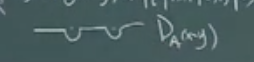
\includegraphics{img/chap3_2.png}
    \caption{第二种围道选择}
    \label{fig3_2}
\end{figure}
然而,不论是推迟Green函数还是超前Green函数,在我们这门课中用途都不是很大,我们经常用到的是下面要介绍的Feynman传播子
\begin{equation}
    D_{F}(x-y)=\int_{C_{F}} \frac{d^{4}p}{(2\pi)^{4}}\frac{i}{p^{2}-m^{2}}e^{-ip(x-y)}
\end{equation}
其选择的围道$C_{F}$如图(\ref{fig3_3})所示。由于我们在这里的积分值完全由极点的位置决定,我们可以稍微移动极点的位置使其位于$\pm(E_{\vec{p}}-i\epsilon)$,其中$\epsilon$是一个无穷小正实数\footnote{这个$\epsilon$被称为Feynman's prescription,它的引入是一个数学上的trick,在任何可观测的物理量结果中不应当出现,因此其具体的取值并不重要。},使得积分路径重新形变成$x$轴,如图(\ref{fig3_4})所示,这样我们可以将Feynman传播子写为
\begin{equation}
\begin{aligned}
     D_{F}(x-y)&=\int \frac{d^{4}p}{(2\pi)^{4}}\frac{i}{p^{2}-m^{2}+i\epsilon}e^{-ip(x-y)}\\
     \widetilde{D}_{F}(p)&=\frac{i}{p^{2}-m^{2}+i\epsilon}\\
     \end{aligned}
\end{equation}
容易验证,Feynman传播子也满足
\begin{equation}
    (\partial^{2}+m^{2})D_{F}(x-y)=-i\delta^{4}(x-y)
\end{equation}
\begin{figure}[htbp]
    \centering
    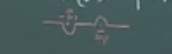
\includegraphics{img/chap3_3.png}
    \caption{Feynman传播子选取的围道}
    \label{fig3_3}
\end{figure}

\begin{figure}[htbp]
    \centering
    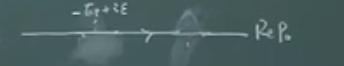
\includegraphics{img/chap3_4.png}
    \caption{形变后的Feynman传播子围道}
    \label{fig3_4}
\end{figure}

从围道选取我们可以看出,不论是$x^{0}>y^{0}$还是$x^{0}<y^{0}$,Feynman传播子都不是0,事实上,当$x^{0}>y^{0}$时
\begin{equation}
    \begin{aligned}
     D_{F}(x-y)&=-\int \frac{d^{3}p}{(2\pi)^{3}}\left.\frac{i^{2}}{2E_{\vec{p}}}e^{-ip(x-y)}\right|_{p^{0}=E_{\vec{p}}}\\
     &=D(x-y)
    \end{aligned}
\end{equation}
当$x^{0}<y^{0}$时
\begin{equation}
    \begin{aligned}
     D_{F}(x-y)&=\int \frac{d^{3}p}{(2\pi)^{3}}\left.\frac{i^{2}}{-2E_{\vec{p}}}e^{-ip(x-y)}\right|_{p^{0}=-E_{\vec{p}}}\\
     &=\int \frac{d^{3}p}{(2\pi)^{3}}\frac{1}{2E_{\vec{p}}}e^{iE_{\vec{p}}t+i\vec{p}\cdot(\vec{x}-\vec{y})}\\
      &=\int \frac{d^{3}p}{(2\pi)^{3}}\frac{1}{2E_{\vec{p}}}e^{-iE_{\vec{p}}t'+i\vec{p}\cdot(\vec{y}-\vec{x})}\\
     &=D(y-x)
    \end{aligned}
    \end{equation}
    其中在第三个等号我们做了变量替换$\vec{q}=-\vec{p}$,并仍将变量名记为$\vec{p}$,同时令$t'=-t=y^{0}-x^{0}$
从而我们有
\begin{equation}
    \begin{aligned}
     D_{F}(x-y)&=\left\{
     \begin{array}{cc}
         D(x-y),\quad x^{0}>y^{0}  \\
          D(y-x),\quad x^{0}<y^{0} \\
     \end{array}
          \right.\\
          &=\theta(x^{0}-y^{0})\bra{0}\phi(x)\phi(y)\ket{0}+\theta(y^{0}-x^{0})\bra{0}\phi(y)\phi(x)\ket{0}\\
          &\doteq\bra{0}T\left[\phi(x)\phi(y)\right]\ket{0}
    \end{aligned}
\end{equation}
最后一行我们引入了编时算符$T$,由定义,编时算符内的场算符是对易的。对于两个算符等时的情况,因为场论保护因果性,从而这两个算符之间的间隔是类空的,从而是可以对易的,其顺序不重要,从而编时算符在等时情况下的定义也是合理的。
对于多个算符我们也可以定义它们的编时乘积
\begin{equation}
    T\left[\phi(x)\phi(y)\phi(z)\right]=\left\{
 \begin{array}{c}
      \phi(x)\phi(y)\phi(z),\quad x^{0}>y^{0}>z^{0}  \\
      \phi(x)\phi(z)\phi(y),\quad x^{0}>z^{0}>y^{0}  \\
       \phi(z)\phi(x)\phi(y),\quad z^{0}>x^{0}>y^{0} \\
       \cdots \\
 \end{array}
    \right.
\end{equation}

后面的课程将会看到,Feynman传播子在利用Feynman图计算散射振幅等方面有着重要应用。事实上,Feynman图内线对应了相应粒子的Feynman传播子。因为今后我们将大量使用Feynman传播子,因此如不特殊说明,我们将Feynman传播子简称为传播子。

